\documentclass[12pt,a4paper]{report}
\usepackage[utf8]{inputenc}
\usepackage[T1]{fontenc}
\usepackage[arabic,english,french]{babel}
\usepackage{geometry}
\usepackage{graphicx}
\usepackage{setspace}
\usepackage{anyfontsize}
\usepackage{fancyhdr}
\usepackage[skip=10pt plus1pt, indent]{parskip}
\usepackage[acronym]{glossaries}
\usepackage[automake]{glossaries-extra}
\usepackage{hyperref}
\usepackage[ruled, linesnumbered]{algorithm2e}
\usepackage{listings}
\usepackage{xcolor}
\usepackage{caption}
\usepackage{subcaption}
\usepackage[numbers]{natbib} 
\usepackage{mathptmx}
\usepackage{array}
\usepackage{multirow}
%*****************************************************************************
\hypersetup{
    colorlinks=true,
    linkcolor=black,
    filecolor=magenta,      
    urlcolor=cyan,
    pdftitle={Overleaf Example},
    pdfpagemode=FullScreen,
    }
    
\urlstyle{same}

%*****************************************************************************
\setstretch{1.5}
%*****************************************************************************

%*****************************************************************************
\setcounter{secnumdepth}{3}
\setcounter{tocdepth}{2}
%*****************************************************************************

%*****************************************************************************
\usepackage{indentfirst}
\addto\captionsfrench{%
\renewcommand*\contentsname{\hfill Table des matières \hfill}
}

\addto\captionsfrench{\renewcommand{\bibname}{Références}}
%*****************************************************************************

%*****************************************************************************
\newgeometry{left=2.54cm,right=2.54cm,top=2.54cm,bottom=2.54cm}
%*****************************************************************************

%*****************************************************************************
\fancypagestyle{plain}{%
  \fancyhf{}%
  \fancyfoot[R]{\thepage}%
  \renewcommand{\headrulewidth}{0pt}
  \renewcommand{\footrulewidth}{0pt}
}

\pagestyle{fancy}
\fancyhead{}
\fancyfoot{}
\fancyfoot[R]{\thepage}
\renewcommand{\headrulewidth}{0pt}
%*****************************************************************************

%*****************************************************************************
\makeglossaries
\newacronym{mi}{MI}{Math et Informatique}
\newacronym{ia}{IA}{Intelligence Artificielle}
%*****************************************************************************

%*****************************************************************************
\definecolor{codegreen}{rgb}{0,0.6,0}
\definecolor{codegray}{rgb}{0.5,0.5,0.5}
\definecolor{codepurple}{rgb}{0.58,0,0.82}
\definecolor{backcolour}{rgb}{0.95,0.95,0.92}

\lstdefinestyle{mystyle}{
    keywordstyle=\color{blue},
    backgroundcolor=\color{backcolour},   
    commentstyle=\color{codegreen},
    numberstyle=\tiny\color{codegray},
    stringstyle=\color{codepurple},
    basicstyle=\ttfamily\footnotesize,
    breakatwhitespace=false,         
    breaklines=true,                 
    captionpos=b,                    
    keepspaces=true,                 
    numbers=left,                    
    numbersep=5pt,                  
    showspaces=false,                
    showstringspaces=false,
    showtabs=false,                  
    tabsize=2
}

\lstset{style=mystyle}
%*****************************************************************************

% \usepackage{titlesec}
% \titleformat{\chapter}[hang]{\normalfont\huge\bfseries}{\chaptertitlename\ \thechapter:}{1em}{}

%*****************************************************************************

\renewcommand{\labelenumii}{\arabic{enumi}.\arabic{enumii}}
\renewcommand{\labelenumiii}{\arabic{enumi}.\arabic{enumii}.\arabic{enumiii}}
\renewcommand{\labelenumiv}{\arabic{enumi}.\arabic{enumii}.\arabic{enumiii}.\arabic{enumiv}}

%*****************************************************************************

\DeclareRobustCommand{\timesr}{\fontfamily{artimes}\selectfont}
\let\times\relax
\DeclareMathSymbol{\times}{\mathbin}{symbols}{"02}

\AtBeginDocument{\def\labelitemi{$\bullet$}}



\begin{document}




\thispagestyle{empty}
\begin{center}
\begin{spacing}{1.15}
République Algérienne Démocratique et Populaire \\
Ministère de l’enseignement Supérieur et de la Recherche Scientifique \\
Université de Mohamed El Bachir El Ibrahimi de Bordj Bou Arréridj\\
Faculté des Mathématiques et d’Informatique\\
Département d'informatique\\
\vspace{0.5cm}


\includegraphics[scale=0.5]{Images/logo.jpeg}

\vspace{0.5cm}

\fontsize{13}{15}\selectfont \textbf{MEMOIRE}\\
Présenté en vue de l’obtention du diplôme \\
\fontsize{13}{15}\selectfont \textbf{Master en informatique} \\
Spécialité: Ajoutez votre spécialité ici 

\vspace{1.5cm}

\fontsize{19}{22}\selectfont \textbf{THEME} \\
\fontsize{19}{22}\selectfont Le thème de ce mémoire ICI
\end{spacing}
\end{center}

\vspace{0.5cm}

\begin{spacing}{1.5}
\noindent
\textit{Présenté par:} \\
NOM ET PRENOM DE L'ETUDIANT 1 \\
NOM ET PRENOM DE L'ETUDIANT 2 \\
~~\\
\textit{Soutenu publiquement le : jj/mm/aaaa} \\
\textit{Devant le jury composé de:} \\
\textbf{Président:} ...................................... \\
\textbf{Examinateur:} ...................................... \\
\textbf{Encadreur:} .................................... \\
\end{spacing}


\centerline{\textbf{2022/2023}}



\pagenumbering{roman}

\chapter*{\hfill Dédicace \hfill}


\vspace{3cm}

\begin{center}
Écrivez votre dédicace ici\\
Une courte dédicace est préférable

\end{center}
\chapter*{\hfill Remerciement \hfill}

\vspace{3cm}

\begin{center}
Gardez-le aussi court et direct que possible.

\end{center}
\chapter*{\hfill Résumé \hfill}

Écrivez votre résumé en français ici. Présentation en quelques lignes du contenu du rapport. Visez 1 paragraphe, mais ne pas dépasser 2 paragraphes. Présentez l'objectif du projet, les résultats obtenus et leur importance.


\chapter*{\hfill Abstract \hfill}

Write your abstract in English here. 

\begin{otherlanguage}{arabic}
\chapter*{\hfill ملخص \hfill}

اكتب ملخصك باللغة العربية هنا
\end{otherlanguage}


\tableofcontents

\cleardoublepage
\addcontentsline{toc}{chapter}{Liste des abréviations}
\printglossary[type=\acronymtype, title={Liste des abréviations}, nonumberlist]
\noindent
(Cette liste est optionnelle, voici un exemple)


\cleardoublepage
\addcontentsline{toc}{chapter}{Liste des figures}
\listoffigures

\cleardoublepage
\addcontentsline{toc}{chapter}{Liste des tableaux}
\listoftables

\cleardoublepage
\addcontentsline{toc}{chapter}{Liste des Algorithmes}
\listofalgorithms

\cleardoublepage

\setcounter{page}{1}
\pagenumbering{arabic}

\chapter{Introduction Générale}
Chaque rapport doit commencer par une introduction générale dans laquelle le contexte du projet est clairement expliqué. Cette introduction devrait également inclure l'objectif du projet et le plan du reste du rapport. Cette introduction ne devrait pas dépasser 2 pages. Soyez concis et clair, et écrivez uniquement ce qui est nécessaire à écrire.

\section{Introduction }
L'évaluation médicale est un processus fondamental dans la pratique clinique, visant à évaluer l'état de santé d'un patient et à déterminer les meilleures stratégies de prise en charge.
 Dans ce contexte, l'Évaluation Médicale Compréhensive (EMC) émerge comme une approche intégrative, cherchant à appréhender la globalité des besoins du patient au-delà de la simple symptomatologie.

\section{Diagnostic médical }
Le diagnostic médical, fruit de la science et de l'expertise, il éclaire le chemin vers la compréhension des symptôme, guidant ainsi le parcours vers la guérison .
\newpage
\subsection{Historique diagnostic }
A ses origines, la médecine était essentiellement magico-religieuse, le diagnostic appartenait aux devins, aux oracles et aux prêtres. Avec Hippocrate, la conception de la médecine devint plus rationnelle et le diagnostic (encore volontiers confondu avec le pronostic) fondé sur un examen clinique minutieux.
Au XVII et au XVIII siècle, la démonstration de la circulation du sang par Harvey introduisit la médecine dans le monde de la mécanique ; Morgagni fonda l’anatomopathologie et la méthode anatomoclinique prit naissance. Son essor se fit dans le cadre du développement de la sémiologie, lui-même lié à la découverte de la percussion à la fin du XVIIIe siècle (Auenbrugger) et à celle de l’auscultation (Laennec) au début du XIX siècle.
Au cours de ce même siècle elle atteignit sa plénitude avec l’apparition de l’anatomopathologie microscopique (Broca). 
A la méthode anatomoclinique vint s’adjoindre avec Claude
Bernard la méthode physio clinique introduisant la physiopathologie et la biologie. Le XIXe siècle vit les débuts de la bactériologie, de l’immunologie et de l’imagerie médicale.
Le XXe siècle fut marqué par le développement de l’endoscopie et des prélèvements biopsiques rendus nécessaires aussi par l’essor de la chirurgie, l’artériographie précédant les méthodes d’explorations non traumatisantes : explorations isotopiques, tomodensitométrie et résonance magnétique nucléaire, l’usage de l’échographie et de l’effet doppler.

La biochimie, la génétique permirent progressivement de substituer à l’étalon or de la confrontation anatomoclinique des critères plus subtils, le passage de l’échelon microscopique au stade de l’échelon moléculaire modifiant progressivement mais radicalement nos conceptions du diagnostic en médecine. Ainsi la médecine des deux derniers siècles a vu se confirmer la rationalité de la démarche médicale puis son développement scientifique, des lésions tissulaires on est passé à la biologie moléculaire.
\subsection{Définitions diagnostic}
Le diagnostic est le processus d'évaluation d'un état de fonctionnement donné. Si cet état est comparé avec un état de référence, il s'agit d'évaluation de dérive de fonctionnement. 
\subsection{Les étapes de diagnostic}

\begin{itemize}
\item \textbf{Collecte d'informations} :
Recueillir des données pertinentes liées au problème ou à la situation, que ce soit des symptômes, des données techniques, des antécédents, etc.

\item \textbf{Identification du problème} :
Analyser les informations collectées pour déterminer la nature du problème. Cela peut impliquer la comparaison des données avec des normes ou des critères établis.

\item \textbf{Élaboration d'hypothèses} :
Formuler des hypothèses sur les causes possibles du problème en se basant sur les informations disponibles.

\item \textbf{Tests et investigations} :
Mettre en place des tests ou des investigations pour valider ou invalider les hypothèses formulées. Cela peut inclure des examens médicaux, des tests techniques, des simulations, etc.

\item \textbf{Analyse des résultats} :
Examiner les résultats des tests et des investigations afin de confirmer la cause du problème ou de revoir les hypothèses si nécessaire.

\item \textbf{Établissement du diagnostic} :
Formuler un diagnostic final en identifiant la cause principale du problème ou de la situation, en tenant compte de toutes les informations et des résultats obtenus.

\item \textbf{Proposition de solutions} :
Proposer des solutions ou des recommandations pour résoudre le problème diagnostiqué. Cela peut impliquer des traitements médicaux, des ajustements techniques, des interventions psychologiques, etc.

\item \textbf{Suivi et évaluation} :
Mettre en place un suivi pour évaluer l'efficacité des solutions proposées et ajuster si nécessaire. Cela peut également inclure des mesures préventives pour éviter la récurrence du problème .

\end{itemize}

\section{Symptômes médicaux  }
Les symptômes médicaux sont souvent les signaux précurseurs d'un état de santé sous-jacent, nécessitant une évaluation médicale approfondie pour établir un diagnostic précis et élaborer un plan de traitement adapté.
\subsection{Définitions les symptômes }
Les symptômes se réfèrent à des signes ou manifestations d'une maladie, d'un trouble ou d'une condition médicale. Ce sont des indicateurs observables ou ressentis par le patient, ainsi que détectés par les professionnels de la santé. Les symptômes médicaux peuvent varier en fonction de la maladie ou du trouble et Il est important de noter que les symptômes ne sont pas la maladie elle-même, mais plutôt des signaux qui indiquent la présence possible d'un problème de santé. Ils peuvent être utilisés pour aider les professionnels de la santé à poser un diagnostic et à recommander un plan de traitement approprié.
\subsection{Exemples de symptômes }
\begin{itemize}
\item La fatigue est définie comme une sensation d'épuisement survenant durant ou après une activité habituelle. Une cause organique ou psychiatrique est retrouvée dans la majorité des cas.

\item Le vomissement est le rejet du contenu de l'estomac par la bouche. Il correspond à un réflexe mécanique de défense de l'organisme destiné à vider l'estomac. Il est possible de vomir des aliments, de la bile ou beaucoup plus rarement, du sang.

\item La fièvre est une température corporelle anormalement élevée, qui dépasse 38°C. 

\item La toux est l'expiration brusque et sonore de l'air contenu dans les poumons provoquée par une irritation des voies respiratoires.

\item La douleur thoracique désigne toute douleur ou toute sensation anormale et pénible localisée dans la zone du thorax.

\item La perte d'appétit est la perte de l'envie de manger, peut aussi être appelée anorexie.

\item Les céphalées sont un problème très courant. Il existe plusieurs types de céphalées, les céphalées de tension étant les plus fréquentes. Bien qu’en général bénignes, les céphalées peuvent être le symptôme d’une maladie grave.
\end{itemize}

\section{Pronostic médical }
Le pronostic médical, étroitement lié aux symptômes médicaux présentés, offre une perspective éclairante sur l'évolution potentielle de la condition de santé, permettant aux professionnels de la santé de prendre des décisions informées pour un plan de traitement optimal.
\subsection{Définition Pronostic médical  }
Le pronostic médical est une évaluation anticipée de l'évolution probable d'une maladie chez un patient, basée sur des données cliniques et des connaissances médicales, afin de prédire les perspectives de guérison, de rémission, de stabilisation ou de progression de la condition.
\subsection{Les type Pronostic médical }
\begin{itemize}
\item \textbf{Pronostic vital} : Il concerne la probabilité de survie d'un patient, souvent exprimée en termes de taux de survie à un certain nombre d'années.

\item \textbf{Pronostic qualité de vie} : Il prend en compte l'impact de la maladie ou du traitement sur la qualité de vie globale du patient.

\item \textbf{Pronostic génétique} : Il se base sur des facteurs génétiques et évalue la probabilité de développement de maladies héréditaires.

\item \textbf{Pronostic fonctionnel} : Il évalue la capacité du patient à maintenir une fonction normale ou à retrouver une fonction normale après un traitement.
\end{itemize}

\section{La relation entre diagnostic, les symptômes et Pronostic médical }
La relation entre le diagnostic, les symptômes et le pronostic médical est cruciale, les symptômes fournissant des indices précieux pour orienter le processus diagnostique, tandis que le diagnostic éclaire le pronostic en permettant une évaluation anticipée de l'évolution probable de la maladie, guider ainsi les choix de traitement et les décisions médicales.
\section{Conclusion}
Cette étude souligne l'interdépendance cruciale entre le diagnostic, les symptômes et le pronostic médical dans le contexte de la médecine moderne. Une compréhension approfondie de ces éléments est essentielle pour assurer des soins de qualité et des résultats positifs pour les patients. 
Le chapitre suivant présente l’apprentissage automatique afin de pouvoir analyser les données médicales.

\chapter{Apprentissage Automatique}

\section{Introduction}
L'apprentissage automatique, en anglais est l'appelé "machine Learning" .
Représente une discipline passionnante au cœur de l'intelligence artificielle. 
Ce domaine cherche à développer des modèles informatiques capables d'apprendre à partir de l'expérience et d'améliorer leurs performances au fil du temps, sans être explicitement programmés.
 

\section{L'apprentissage Automatique }
L’apprentissage automatique est un type d'intelligence artificielle (IA), c’est une science qui permet aux ordinateurs d'apprendre sans être explicitement programmés « Arthur Samuel, 1959 ». Plus précisément, l'apprentissage automatique fait référence au développement, l'analyse et l'implémentation de méthodes qui permettent à une machine (au sens large) d'évoluer et de remplir des tâches associées à une intelligence artificielle grâce à un processus d'apprentissage. Cet apprentissage permet d'avoir un système qui s'optimise en fonction de l'environnement, les expériences et les résultats observés.
Dans le domaine médicale, l’apprentissage automatique a été conçu pour réaliser l'analyse de données médicales, surtout lorsque l'évolution numérique a fourni des moyens (capteurs) peu coûteux permettant de recueillir et de stocker des informations importantes liées aux patients et maladies. Par exemple, les algorithmes d'apprentissage sont utiles au médecin lors du diagnostic des patients, afin d'améliorer la vitesse, la précision et la fiabilité de son diagnostic.

\section{Types d’Apprentissage Automatique }
Il existe fondamentalement quatre types d’apprentissage automatique : Supervisé, semi-supervisé et non-supervisé et Apprentissage par renforcement. 
Dans notre étude, nous utilisons l’apprentissage supervisé pour construire des modèles pour la prédiction des maladies.
Dans la suite de cette section, nous allons présenter les deux types d’apprentissage les plus utilisés qui sont l’apprentissage supervisé et apprentissage non supervisé.

\begin{figure}[h]
\centering
\includegraphics[scale=0.8]{Images/Chapiter2/Types d’Apprentissage Automatique.PNG}
\caption{Les différentes méthodes d'apprentissage automatique.}
\label{fig:01}
\end{figure}

\subsection{Apprentissage Supervisé }
Dans l'apprentissage supervisé, l'ordinateur est fourni avec des exemples d'entrées qui sont étiquetés avec les sorties souhaitées. Le but de cette méthode est que l'algorithme puisse « apprendre » en comparant sa sortie réelle avec les sorties « apprises » pour trouver des erreurs et modifier le modèle en conséquence. 
L'objectif des algorithmes d'apprentissage supervisé est d'apprendre une fonction qui mappe les vecteurs de caractéristiques (entrées) aux étiquettes (sortie), sur la base d'exemples de paires entrée-sortie.  

Comme il est illustré dans la Figure 1 l’apprentissage supervisé peut être utilisé pour deux types de tâches principales : la classification et la régression. 
Les algorithmes de classification cherchent à prédire la classe ou la catégorie à laquelle appartient une donnée d'entrée tandis que les algorithmes de régression servent à prédire une valeur numérique continue à partir de variables d'entrée. Dans ce travail, nous nous intéressons aux méthodes de classification.
\subsection{Apprentissage Non-Supervisé  }
Dans l'apprentissage non supervisé, les données sont non étiquetées, de sorte que l'algorithme d'apprentissage trouve tout seul des points communs parmi ses données d'entrée. Les données non étiquetées étant plus abondantes que les données étiquetées, les méthodes d'apprentissage automatique qui facilitent l'apprentissage non supervisé sont particulièrement utiles.
L'objectif de l'apprentissage non supervisé peut être aussi simple que de découvrir des modèles cachés dans un ensemble de données.
Les plus fréquents problèmes connus dans ce type sont :
\begin{itemize}
\item Le clustering qui consiste à regrouper un ensemble d’éléments hétérogènes sous forme de sous-groupes homogènes.

\item La réduction de dimension qui consiste à prendre des données dans un espace de grande dimension, et à les remplacer par des données dans un espace de plus petite dimension sans perdre la variance .
\end{itemize}


\section{Définition de classification }
Un modèle de classification est un modèle d'apprentissage automatique qui attribue des étiquettes ou des catégories à des instances d'entrée en les associant à un ensemble fini de classes prédéfinies. 
L'objectif est de créer une fonction qui peut généraliser à de nouvelles données et assigner correctement des classes à des observations inconnues en fonction des modèles appris à partir des données d'entraînement. 
Les classes peuvent être binaires (deux classes, comme oui/non) ou multinomiales (plus de deux classes), et le modèle cherche à discriminer entre ces classes en fonction des caractéristiques des données d'entrée.

\section{Les types de classification }
Dans cette partie, nous présentons les types de classification :
\newpage
\subsection{La classification binaire (Binary classification) }
La classification binaire (ou la classification binomiale) est une transformation de données qui vise à répartir les membres d'un ensemble dans deux groupes disjoints selon que l'élément possède ou non une propriété / fonctionnalité donnée, mais peut également être interprété comme vrai et faux, 1 et 0, ou toute autre combinaison de deux valeurs. 
Par exemple : tests médicaux visant à déterminer si un patient est atteint d'une certaine maladie ou non. 

\begin{figure}[!h]
\centering
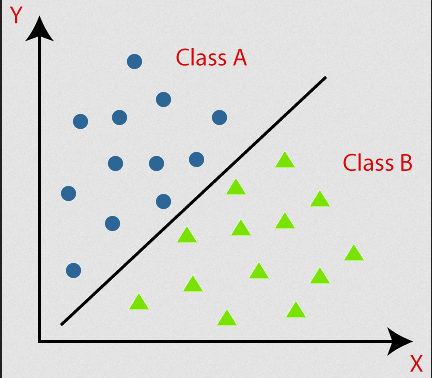
\includegraphics[scale=0.5]{Images/Chapiter2/La classification binaire.png}
\caption{Exemple de problème de classification binaire.}
\label{fig:02}
\end{figure}

\begin{itemize}
\item L’image montre qu’il y a deux classes : classe A et classe B.
\end{itemize}
\begin{center}
\end{center}


\subsection{La classification multi-classe }
La classification multi-classe désigne une tâche de classification comportant plus de deux classes, par exemple, La classification des visages, classification des espèces végétales...Ect.
 Un jeu de données multi-classe n’a qu’une seule classe en sortie, comme dans la classification binaire.
 \newpage

\subsection{La classification multi-lable }
Jusqu'à présent, chaque instance était toujours affectée à une seule classe. Dans certains cas, le classificateur peut produire plusieurs classes pour chaque instance.
   Par exemple, un classificateur pour reconnaître des types de maladies : que faire s'il reconnaît plusieurs symptômes en même temps ? Bien entendu, il doit noter chaque symptôme associé à une maladie spécifique. Supposons qu'un classificateur ait été formé pour reconnaître trois symptômes : « fatigue, nausée et température élevée ».
Ainsi, lorsqu’il apparaît « fatigué et une forte température ».
Il devrait produire [1, 0, 1] (c'est-à-dire : fatigué oui, nausée non, fièvre oui.) Un système de classification qui produit plusieurs binaires est appelé système de classification multi-étiquettes.

\begin{figure}[!h]
\centering
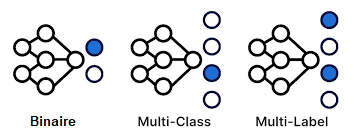
\includegraphics[scale=1]{Images/Chapiter2/La classification multi-lable.png}
\caption{Exemple de problème de classification binaire , multi-classe et multi-lable .}
\label{fig:03}
\end{figure}

\section{Techniques de Classification }
Dans cette partie, nous présentons les algorithmes de classification :

\subsection{Les k plus proches voisins (KNN) }
L’algorithme des k plus proches voisins en anglais est l'appelé « K-Nearest Neighbors (KNN) » est un algorithme de classification supervisé. Chaque observation de l’ensemble d’apprentissage est représentée par un point dans un espace à n dimensions ou n est le nombre de variables prédictives. Pour prédire la classe d’une observation, on cherche les k points les plus proches de cet exemple. La classe de la variable cible, est celle qui est la plus représentée parmi les k plus proches voisins. Il existe des variantes de l’algorithme ou on pondère les k observations en fonction de leur distance à l’exemple dont on veut classer les observations les plus éloignées de notre exemple seront considérées comme moins importantes.

\begin{figure}[!h]
\centering
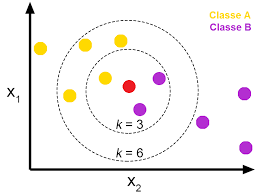
\includegraphics[scale=0.8]{Images/Chapiter2/Les k plus proches voisins (KNN).png}
\caption{Pour k = 3 la classe majoritaire du point central est la classe B, mais si on change la valeur du voisinage k = 6 la classe majoritaire devient la classe A .}
\label{fig:03}
\end{figure}

\subsection{k-means }
L’algorithme des k-moyennes en anglais est l'appelé « k-means » est un algorithme non supervisé. Chaque observation est représentée par un point dans un espace à n dimensions ou n est le nombre de variables descriptives.
À partir d’un ensemble d’apprentissage de $M$ observations $[X^{1}, \ldots, X^{M}]$ cet algorithme va repartir ces observations en k clusters de manière à ce que la distance euclidienne qui sépare les points au centre de gravité du groupe auquel ils sont affectés soit minimale. Les étapes de l’algorithme sont :

\begin{itemize}
\item Choisir k points qui représentent la position moyenne des clusters.
\item répéter jusqu’à stabilisation des points centraux :
\begin{itemize}
\item[-] affecter chacun des M points au plus proche des k points centraux.
\item[-]mettre à jour les points centraux en calculant les centres de gravité des k cluster.
\end{itemize}
\end{itemize}

\begin{figure}[!h]
\centering
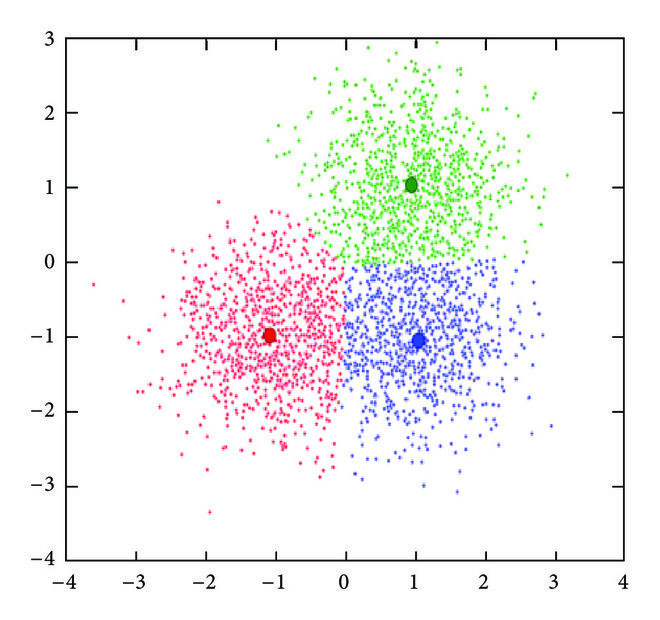
\includegraphics[width=8cm, height=6cm]{Images/Chapiter2/k-means.png}
\caption{L’algorithme k-means regroupe les données en k cluster, ici k = 3. Les centres de gravité sont représentés par de petit cercle.}
\label{fig:04}
\end{figure}

\subsection{Régression Logistique}
L'analyse de régression est souvent utilisée pour faire des prédictions, comprendre les variables indépendantes par rapport à la variable dépendante et étudier la forme de leur relation.
Dans des circonstances limitées, l'analyse de régression peut être utilisée pour déduire la relation causale entre la variable indépendante et la variable dépendante.
La régression est un algorithme robuste lorsqu'il s'agit de classer des ensembles de problèmes, et a une fonction logistique (fonction sigmoïde) au cœur de celui-ci. Dans cet algorithme, les valeurs d'entrée sont combinées en fonction de coefficients ou de poids pour donner les valeurs de sortie/prédites. 

\begin{figure}[!h]
\centering
\includegraphics[scale=1]{Images/Chapiter2/Régression Logistique .png}
\caption{Modèle la régression logistique.}
\label{fig:05}
\end{figure}
\newpage
\subsection{Machine à Vecteurs de Supports (S V M) }
Machine à Vecteurs de Supports en anglais cela l'appelé « Support Vector Machine » est l’un des algorithmes d’apprentissage supervisé les plus populaires, utilisé pour les problèmes de classification et de régression. 
Cependant, il est principalement utilisé pour les problèmes de classification dans l’apprentissage automatique. Le but de l’algorithme SVM est de créer la meilleure ligne ou limite de décision qui peut séparer l’espace à n dimensions en classes afin que nous puissions facilement mettre le nouveau point de données dans la bonne classe à l’avenir.

\begin{figure}[!h]
\centering
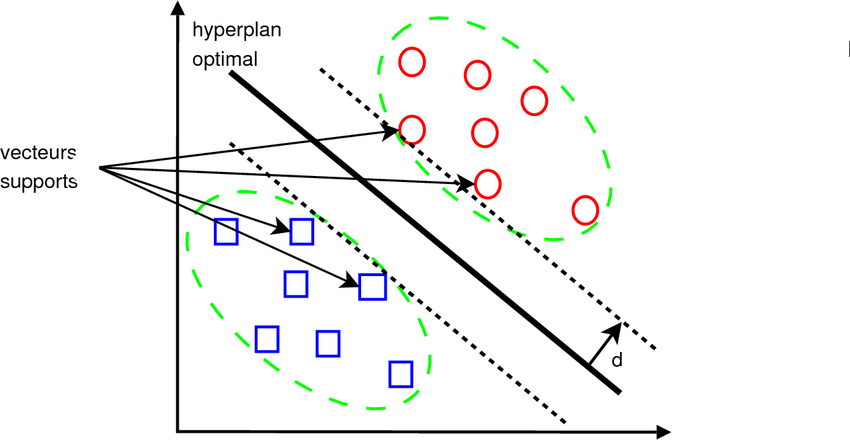
\includegraphics[scale=0.5]{Images/Les-vecteurs-de-support.png}
\caption{Un diagramme d'un hyperplan avec des vecteurs de support dans un espace vectoriel à deux dimensions.}
\label{fig:06}
\end{figure}


\begin{itemize}
\item[-] La figure \ref{fig:06} montre un exemple simple d'un hyperplan avec des vecteurs de support. Cette technique peut être utilisée pour séparer deux classes de points dans un espace vectoriel, ce qui est utile pour des tâches d'apprentissage automatique telles que la classification et la régression.
L'objectif d'un hyperplan avec des vecteurs de support est de trouver la meilleure séparation possible entre deux classes de points dans un espace vectoriel. Cela peut être utilisé pour des tâches de classification, telles que la reconnaissance d'image ou le traitement du langage naturel.
\end{itemize}

\subsection{Apprentissage profondeur }
Apprentissage profond en anglais est l'appelé « Deep Learning » est un type d'intelligence artificielle dérivé du machine Learning (apprentissage automatique) où la machine est capable d'apprendre par elle-même, contrairement à la programmation où elle se contente d'exécuter à la lettre des règles prédéterminées.

\begin{figure}[h]
\centering
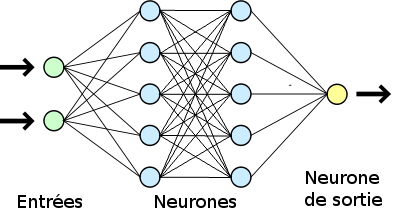
\includegraphics[scale=0.8]{Images/Chapiter2/Apprentissage profondeur.png}
\caption{Architecture Apprentissage profondeur.}
\label{fig:07}
\end{figure}

La figure \ref*{fig:07} fournie montre une architecture d'apprentissage profond composée de plusieurs couches empilées les unes sur les autres. Chaque couche est composée d'un certain nombre de neurones artificiels qui sont interconnectés. 
Les neurones sont responsables de traiter les informations et de les transmettre à la couche suivante.

\begin{itemize}
\item \textbf{Couches d'entrée} : Elles reçoivent les données brutes, comme des images ou du texte.
\item \textbf{Couches cachées} : Elles traitent les données et extraient des caractéristiques de plus en plus complexes.
\item \textbf{Couche de sortie} : Elle produit la sortie finale, comme une classification ou une prédiction.
\end{itemize}

\newpage
\section{Comparaison entre techniques de classification}

\label{tab:01}
\begin{table}[h]

\begin{tabular}{| m{3cm}| m{6cm}| m{6cm}|}
\hline
 \textbf{Techniques de Classification} & \textbf{Avantages} & \textbf{Inconvénients} \\ 
 \hline
 \textbf{KNN} & - Simple à concevoir &
 \begin{itemize}
 \item[-]Sensible aux bruits.
 \item[-]Pour un nombre de variable prédictives très grands, le calcul de la distance devient très coûteux.
 \end{itemize}
 
 \\  
 \hline
\textbf{ k-means} & -implémentable pour des grands volumes de données & 
 \begin{itemize}
 \item[-]Le choix du paramètre k n’est pas découvert mais choisi par l’utilisateur .
 \item[-] La solution dépend des k centre de gravité choisi lors de l’initialisation
 \end{itemize}
 \\
 \hline
 \textbf{Régression Logistique} & - Ses résultats sont faciles à interpréter. & 
 \begin{itemize}
\item[-] La phase d’apprentissage peut être longue car l’optimisation des coefficients est complexe. 
\item[-]Sa linéarité empêche la prise en compte des interactions entre les variables.
\end{itemize}
 \\
 \hline
 \textbf{S V M} &
 \begin{itemize} 
 \item[-]Il permet de traiter des problèmes de classification non linéaire complexe.
 \item[-]Les SVM constituent une alternative aux réseaux de neurones car plus faciles à entraîner.
 \end{itemize}
 & 
 \begin{itemize} 
 \item[-] Les SVM peuvent être lents à entraîner sur de grands ensembles de données.
 \item[-] Cela peut affecter la précision du modèle et le rendre moins fiable.
 \end{itemize}
 \\
 \hline
 \textbf{Apprentissage profondeur} &
 \begin{itemize}
  \item[-] Adaptabilité à Divers Domaines.
  \item[-] Performances Exceptionnelles dans des Tâches Complexes.
  
  \end{itemize}
 & 
 \begin{itemize}
 \item[-]Interprétabilité Limitée.
 \item[-]Besoin d'Expertise Technique Élevée.
 
 \end{itemize}
\\
 \hline
\end{tabular}
\end{table}

\newpage
\section{Conclusion}
Dans ce chapitre, nous avons présenté les algorithmes d'apprentissage supervisé. 
Après avoir présenté les deux principaux types d’apprentissage automatique, une description détaillée de chaque méthode de classification a été fournie, en expliquant le principe de fonctionnement de chaque méthode ainsi que ses avantages et inconvénients.
Le chapitre suivant présente les méthodes d’apprentissage profondeur qui ont été appliquées dans le domaine de la santé.

\chapter{Deep Learning}

\section{Introduction }
L’apprentissage profond ou le deep Learning est un nouveau domaine de recherche du Machine Learning(ML), qui a été introduit dans le but de rapprocher le ML de son objectif principal : l’intelligence artificielle.
 Il concerne les algorithmes inspirés par la structure et le fonctionnement du cerveau. 
 Ils peuvent apprendre plusieurs niveaux de représentation dans le but de modéliser des relations complexes entre les données.
 
 \begin{figure}[h]
\centering
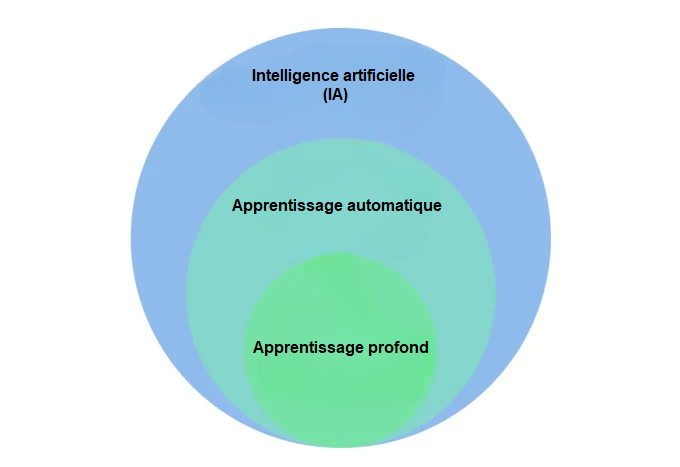
\includegraphics[scale=0.9]{Images/ia reglo.png}
\caption{La relation entre l’intelligence artificielle, le Machine L earning et le deep learning.}
\label{fig:08}
\end{figure} 
 
 \section{L’apprentissage profond }
 L'apprentissage profond est une technologie d'intelligence artificielle révolutionnaire qui permet aux machines d'apprendre à partir de données massives, ouvrant ainsi la voie à des avancées majeures. Malgré ses succès, il présente des défis, mais continue de repousser les frontières de l'intelligence artificielle.
 
\subsection{Définition l'apprentissage profond}
L’apprentissage profond en anglais cet appelée «Deep Learning » une technique d'apprentissage automatique révolutionnaire qui a permis de réaliser des progrès importants dans de nombreux domaines tels que la vision par ordinateur, la reconnaissance de la parole et la traduction automatique. 
Grâce à sa capacité à apprendre par elle-même et à résoudre des problèmes complexes, l'apprentissage profond est un outil puissant qui continuera à jouer un rôle majeur dans l'évolution de l'intelligence artificielle. 

\subsection{Domaines d'application de l'apprentissage profonde }
Le deep Learning utilisé dans plusieurs domaines différents tels que :

\begin{itemize}
\item  \textbf{Traitement du langage naturel (NLP)} : L'apprentissage profond est employé dans la compréhension du langage naturel, la traduction automatique, la génération de texte, la classification de texte, et l'analyse des sentiments.

\item \textbf{Santé} : L'apprentissage profond est appliqué dans le diagnostic médical, la segmentation d'images médicales, la prédiction de maladies, et la découverte de médicaments.

\item \textbf{Vision par ordinateur} : L'apprentissage profond est largement utilisé pour la reconnaissance d'images, la segmentation d'images, la détection d'objets, la classification d'images, et la génération d'images.

\item \textbf{Robotique} : L'apprentissage profond est employé dans la perception sensorielle des robots, la planification de mouvements, et l'interaction homme-robot.
\end{itemize}

 \section{Principes de fonctionnement }
 D’apprentissage en profondeur sont formés sur la base des structures de données complexes qu'ils rencontrent. 
Ils construisent des modèles informatiques composés de plusieurs couches (couche d'entrée, couche cachée, couche de sortie) de traitement pour créer plusieurs niveaux d'abstraction pour représenter les données. 

\begin{figure}[h]
\centering
\includegraphics[scale=0.8]{Images/réseau.png}
\caption{les couches d’apprentissage profond.}
\label{fig:09}
\end{figure}

\subsection{Les types des couches dans d’apprentissage profond}

\begin{itemize}
\item  \textbf{Couche d’entrée} : composée d’un ensemble de neurones qui favoriseront la propagation des informations dans le réseau neuronal. Elle comprend un nombre de neurones généralement égal au nombre de caractéristiques constituant l’enregistrement en entrée (p. ex. une image, une transaction, etc.).
\item \textbf{Couches intermédiaires} : servant à traiter l’information propagée dans le réseau de neurones pour capturer les caractéristiques de son apprentissage.
\item \textbf{Couche de sortie} : formée d’un ensemble de neurones représentant les différentes classes de résultat.
 Dans une problématique de classification, les classes sont les différentes possibilités que le résultat peut offrir.
 
\end{itemize}

 \section{Les poids }
 \label{Les poids}
 Les poids des flèches sont utilisés pour accorder de l'importance à certaines fonctionnalités par rapport à d'autres, afin d'obtenir les résultats souhaités. La somme pondérée de tous les poids des flèches est calculée pour chaque neurone d'une couche cachée, et chacun de ces neurones exécute une fonction d'activation qui lui est propre.

 \section{La fonction d'activation }
 Une fonction d’activation, qui associe à chaque valeur agrégée une unique valeur de sortie dépendant du seuil.
 
 \begin{figure}[h]
\centering
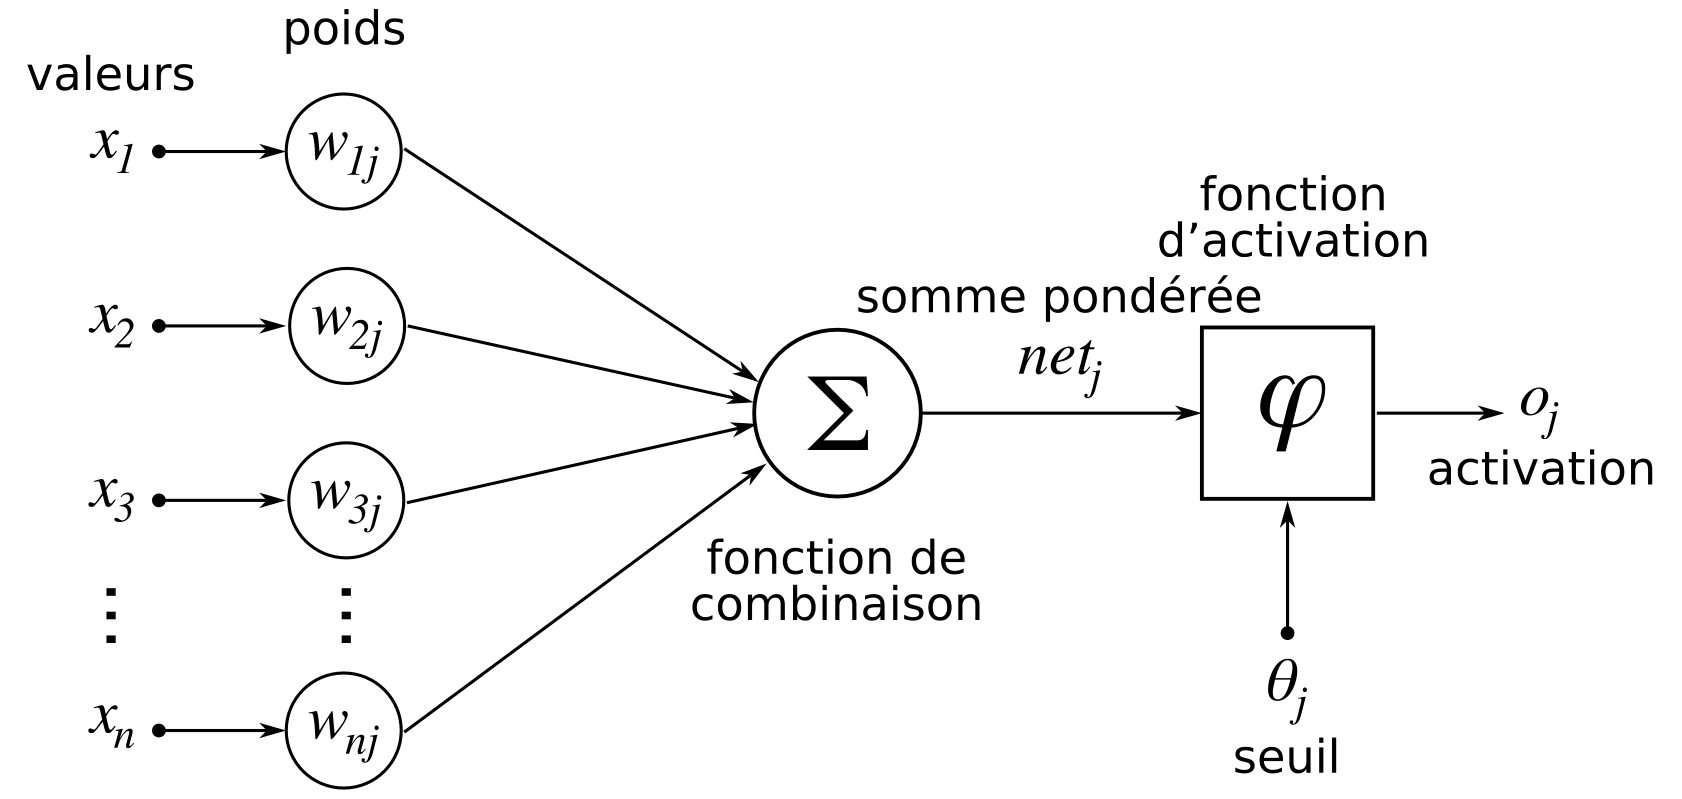
\includegraphics[scale=0.3]{Images/1-neurone-formel.png}
\caption{Fonction d’activation.}
\label{fig:10}
\end{figure}

\subsection{La fonction Relu }

La fonction Unité Linéaire Rectifiée en anglais, appelée Rectified Linear Unit (ReLU), est la fonction d'activation la plus couramment utilisée en Deep Learning. Elle est définie comme suit :

\[ \text{ReLU}(x) = \max(x, 0) \]

Cette fonction renvoie $x$ si $x$ est supérieur à 0, et 0 sinon. Autrement dit, elle calcule le maximum entre $x$ et 0.


\begin{figure}[h]
\centering
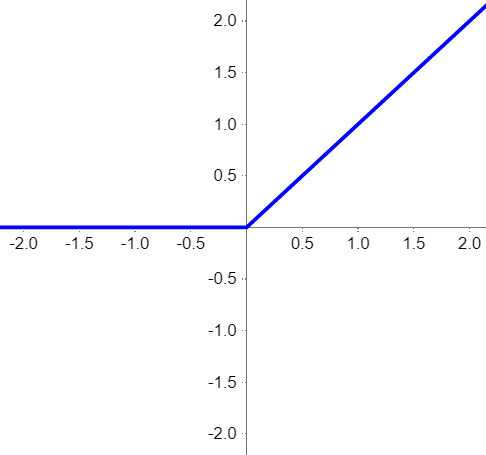
\includegraphics[scale=0.5]{Images/relu.png}
\caption{La fonction Relu.}
\label{fig:11}
\end{figure}

Cette fonction permet d’appliquer un filtre en sortie de couche. 
Elle laisse passer les valeurs positives dans les couches suivantes et bloque les valeurs négatives. 
Ce filtre permet alors au modèle de se concentrer uniquement sur certaines caractéristiques des données, les autres étant éliminées.

\subsection{La fonction d'un softmax }
La fonction Softmax est la fonction d'activation utilisée en dernière couche d'un réseau de neurones construit pour effectuer une tâche de classification multi-classes. Pour chaque sortie, Softmax donne un résultat entre 0 et 1. De plus, si l'on additionne ces sorties entre elles, le résultat donne 1.

La fonction Softmax est définie mathématiquement comme suit :

\[ \text{Softmax}(x) = \frac{e^{x}}{\sum_{i} e^{x_i}} \]


\begin{figure}[h]
\centering
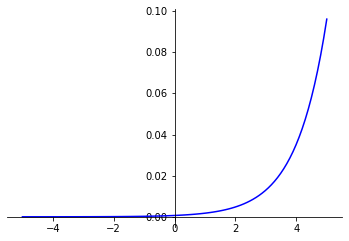
\includegraphics[scale=0.5]{Images/Softmax.png}
\caption{La fonction d'un softmax.}
\label{fig:12}
\end{figure}

La fonction Softmax, grâce à sa caractéristique de produire des résultats qui, additionnés, donnent 1, respecte les lois de probabilité. Elle est donc le noyau dur d’un réseau de neurones construit pour effectuer une tâche de classification multi-classes.

\subsection{La fonction sigmoïde }
La fonction sigmoïde est la fonction d'activation utilisée en dernière couche d'un réseau de neurones construit pour effectuer une tâche de classification binaire. Elle donne une valeur entre 0 et 1.

La fonction sigmoïde est définie mathématiquement comme suit :

\[ \text{Sigmoid}(x) = \frac{1}{1 + e^{-x}}\]
\begin{figure}[h]
\centering
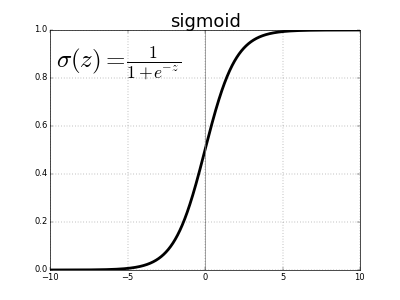
\includegraphics[scale=0.5]{Images/sigmoid.png}
\caption{La fonction sigmoïde.}
\label{fig:13}
\end{figure}

Cette valeur peut être interprétée comme une probabilité. Dans une classification binaire, la fonction d’activation sigmoïde permet alors d’obtenir, pour une donnée, la probabilité d’appartenir à une classe.
Dans cet exemple, plus le résultat de la sigmoïde est proche de 1, plus le modèle considère que la critique est positive. Inversement, plus le résultat de la sigmoïde est proche de 0, plus le modèle considère que la critique est négative.
La fonction d’activation sigmoïde permet donc d’obtenir un résultat ambivalent, donnant une indication sur deux classes à la fois.

\section{Les différents types de model deep Learning}
On va présenter dans cette section les modèles de deep Learning utilisés dans notre proposition à savoir les CNN, RNN, LSTM et ANN.

\subsection{Le réseau de neurone convolutif (CNN) }
Le nom ‘Réseau de neurones à convolution’ indique que le réseau emploi une opération mathématique appelée la convolution.
 Les réseaux de convolution sont un type spécialisé de réseaux neuronaux qui utilisent la convolution à la place de la multiplication matricielle générale dans au moins une de leurs couches.
 Les CNN sont l’un des meilleurs algorithmes d’apprentissage pour faire l’opération de convolution qui aide à l’extraction de fonctionnalités utiles à partir de points de données corrélés localement.
 La sortie des noyaux convolutifs est ensuite affectée à l’unité de traitement non linéaire (fonction d’activation), qui non seulement aide à apprendre les abstractions, mais intègre également la non-linéarité dans l’espace des fonctionnalités.

\begin{figure}[!h]
\centering
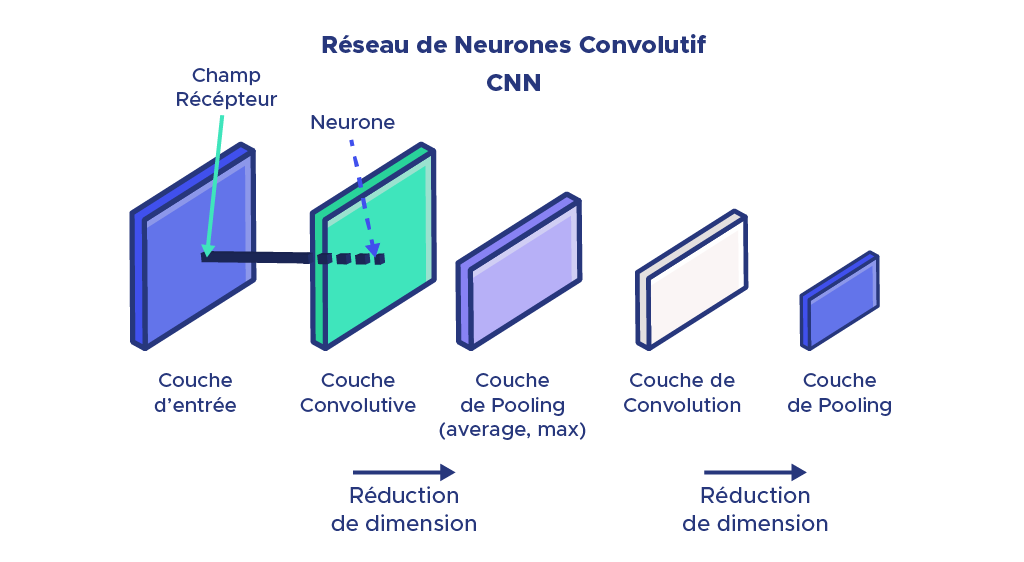
\includegraphics[width=13cm, height=6cm]{Images/illu_DenseNet-09.png}
\caption{Structure générale d’un réseau CNN.}
\label{fig:14}
\end{figure}
\newpage
\subsection{Réseau de neurones récurrents (RNN) }
Un réseau de neurones récurrent (RNN, Recurrent Neural Network) est un type de réseau de neurones artificiels principalement utilisé dans la reconnaissance vocale et le traitement automatique du langage naturel et la traduction automatique.
Les RNN sont conçus de manière à reconnaître les caractéristiques séquentielles et les modèles d'utilisation des données requis pour prédire les scénarios faisant intervenir le contexte dans la prédiction d'un résultat . 

\begin{figure}[!h]
\centering
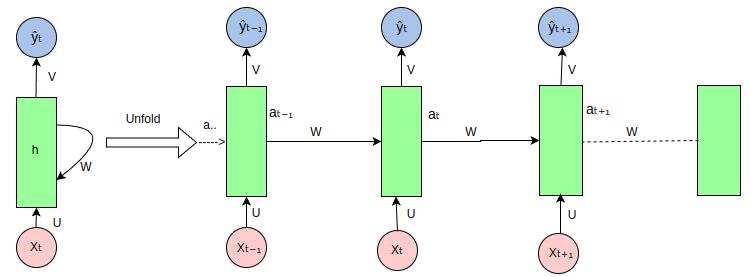
\includegraphics[scale=0.6]{Images/1_dznTsiaHCvRc70fxWWEcgw.png}
\caption{Architecture de RNN.}
\label{fig:15}
\end{figure}
\newpage
\subsection{Les réseaux LSTM }
Les réseaux mémoire à long terme (LSTM : Long Short-Term Memory, en anglais) sont des dérivés de RNN. Ils peuvent apprendre et mémoriser des dépendances sur une longue durée. Les LSTM conservent ainsi les informations mémorisées sur le long terme. Ils sont particulièrement utiles pour prédire des séries chronologiques, car ils se rappellent des entrées précédentes. Outre ce cas d'utilisation, les LSTM sont également utilisés pour composer des notes de musique et reconnaître des voix.

\begin{figure}[!h]
\centering
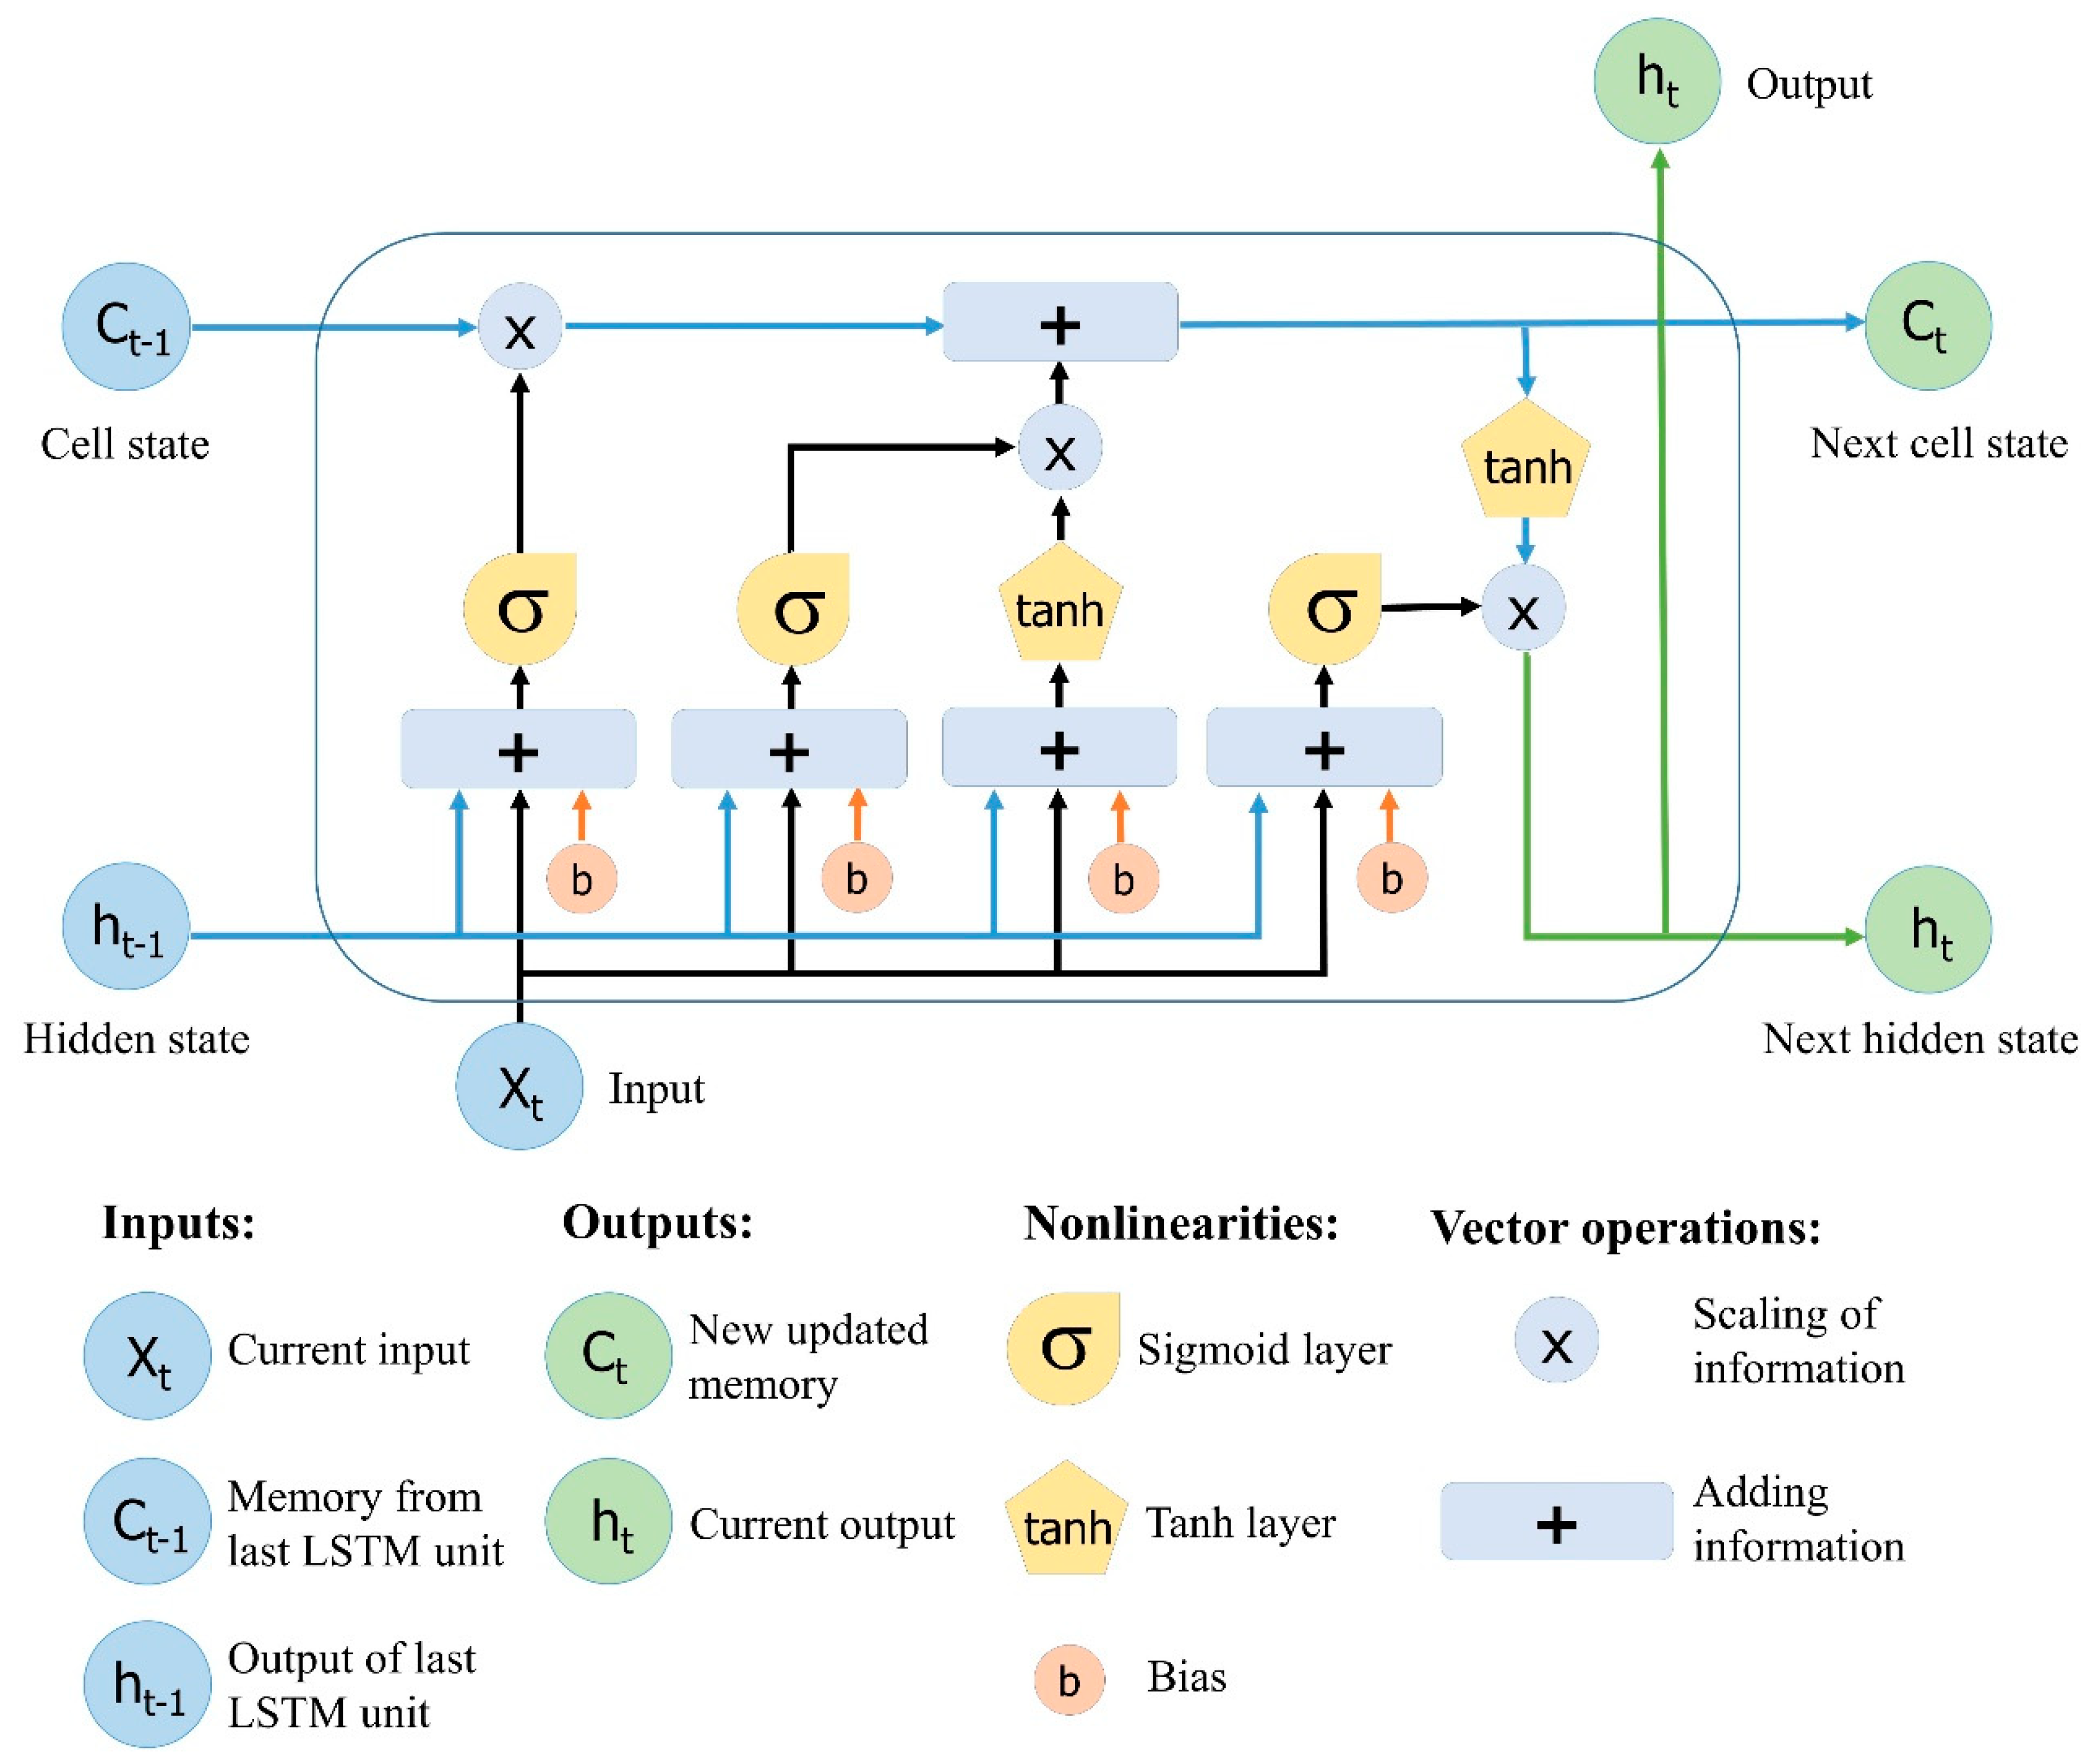
\includegraphics[scale=0.1]{Images/water-11-01387-g004.png}
\caption{Le module répétitif dans un LSTM.}
\label{fig:16}
\end{figure}
\newpage
\subsection{Réseaux de neurones artificiel (ANN) }
C’est une structure constituée de suite successive de couches de nœuds et qui permet de définir une fonction de transformation non linéaire des vecteurs d’entrées (composés dans le cas de classification des mots pondérés de leur poids) en vecteur de catégories. 
 La disposition des neurones dans le réseau ainsi que le nombre de couches utilisées ont une influence sur le résultat de classification.
Comparés aux autres méthodes de classification par apprentissage supervisé, les réseaux de neurones artificiels sont habituellement utilisés pour des tâches de classification. 
Par analogie avec la biologie, ces unités sont appelées neurones formels.
Un neurone formel est caractérisé par :

\begin{itemize}
\item Le type des entrées et des sorties.
\item Une fonction d’entrée.
\item Une fonction de sortie.
\end{itemize}

\begin{figure}[!h]
\centering
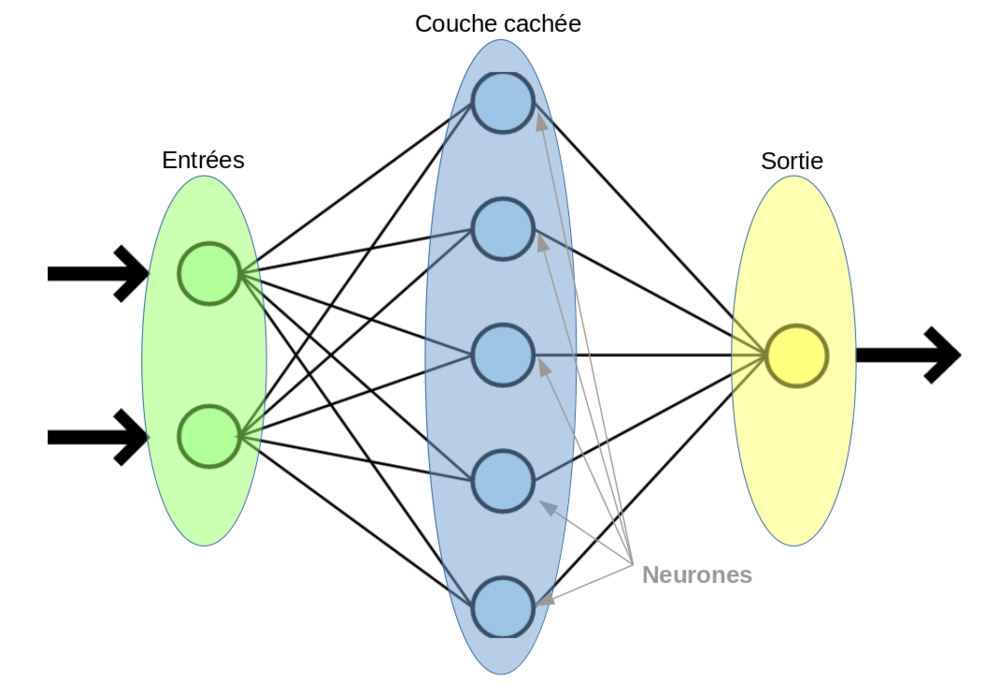
\includegraphics[scale=0.3]{Images/ANN.png}
\caption{Architecture de réseau de neurones artificiels.}
\label{fig:17}
\end{figure}

\newpage
\section{ Conclusion }

Dans ce chapitre nous avons présenté l'apprentissage en profondeur (DL) et ses différents types de réseaux de neurones artificiels : les réseaux de neurones artificiels (ANN), les réseaux de neurones convolutifs (CNN) et les réseaux de neurones récurrents (RNN), y compris les réseaux à mémoire longue durée (LSTM).

Le chapitre suivant se concentre sur l'expérimentation de la construction de modèles de réseaux de neurones artificiels avec compression de données utilisant l'algorithme des composantes principales (PCA). 
Nous appliquerons également différents types d'algorithmes d'optimisation.



\chapter{Figures, tableaux et références}

\section{...}
Chaque figure et chaque tableau doit être référencé. L'ajout des figures et des tableaux à l'aide du \LaTeX\ est simple. Ce chapitre présente quelques exemples de ce processus d'ajout.

\section{Les tableaux}
Le lien suivant explique en détail la manière avec laquelle doit être faite la création et la personnalisation des tableaux à l'aide du \LaTeX\ : \url{https://fr.overleaf.com/learn/latex/Tables}

Le tableau \ref{tab:01} illustre un exemple d'un tableau.

\begin{table}[h]
\centering
\caption{Un exemple d'un tableau.}
\label{tab:01}
\begin{tabular}{|c|c|c|}
\hline
 \textbf{Methods} & \textbf{Result 1} & \textbf{Result 2} \\ 
 \hline
 \textbf{Method 1} & 0.67 & 0.74 \\  
 \hline
 \textbf{Method 2} & 0.86 & 0.90 \\
 \hline
\end{tabular}
\end{table}


\section{Les figures}
Veuillez vous référer au lien suivant pour une description détaillée sur la façon d'insérer des images dans votre document \LaTeX\ et la façon de les référencer dans le texte: \url{https://fr.overleaf.com/learn/latex/Inserting_Images}

La figure \ref{fig:01} illustre une figure qui a été ajoutée juste pour montrer un exemple et la figure \ref{fig:02} illustre une figure principale avec deux sous-figures \ref{fig:02a} and \ref{fig:02b}.

\begin{figure}[h]
\centering
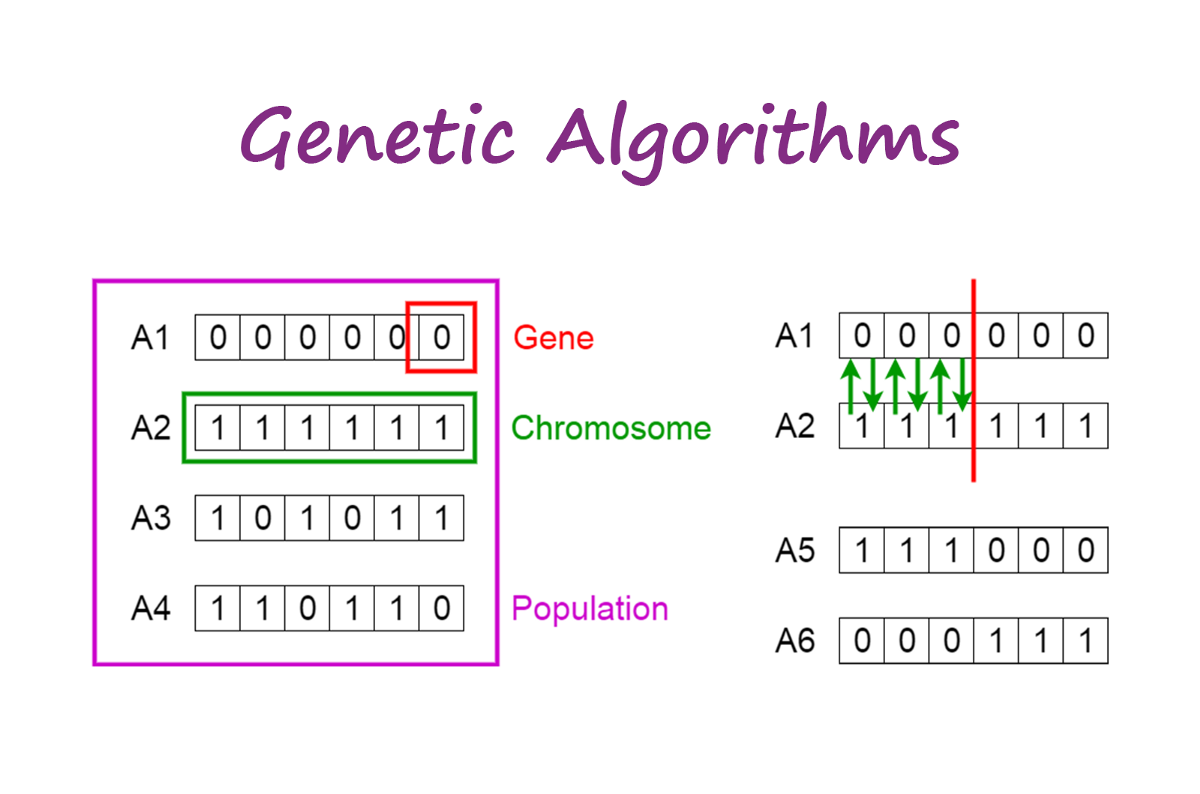
\includegraphics[scale=0.3]{Images/Chapter4/GeneticAlgorithm.png}
\caption{Un exemple d'une figure.}
\label{fig:01}
\end{figure}

~~\\
~~\\



\begin{figure}[h]
     \centering
     \begin{subfigure}[b]{0.4\textwidth}
         \centering
         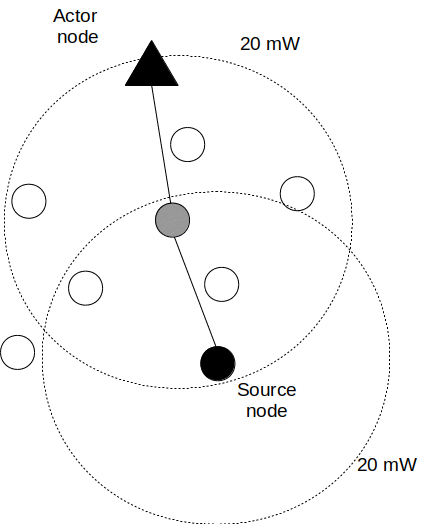
\includegraphics[scale=0.40]{Images/Chapter4/ExempleSansAjustement.png}
         \caption{}
         \label{fig:02a}
     \end{subfigure}
     \hfill
     \begin{subfigure}[b]{0.4\textwidth}
         \centering
         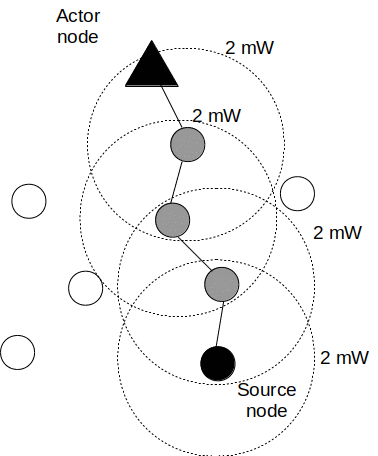
\includegraphics[scale=0.40]{Images/Chapter4/ExempleAvecAjustement.png}
         \caption{}
         \label{fig:02b}
     \end{subfigure}
     \hfill
    \caption{Un exemple d'une figure avec deux sous-figures.}
    \label{fig:02}
\end{figure}

~~\\


\section{Les références}
Les listes de références sont gérées en \LaTeX\ à l'aide de l'outil Bib\TeX\, logiciel de gestion de références bibliographiques développé principalement à cet effet. Voici le lien suivant qui explique en détail comment utiliser Bib\TeX\ :  \url{https://fr.overleaf.com/learn/latex/Bibliography_management_with_bibtex}

Veuillez suivre le style de référence IEEE, pour cela, vous pouvez choisir, par exemple, le style de référence \verb|IEEEtranN|, ce dernier qui nécessite l'invocation du package \verb|natbib| en ajoutant \verb+\usepackage[numbers]{natbib}+ au préambule.

\cite{4}, \cite{2}, \cite{3}, \cite{5}, \cite{1}, ...


\section{...}
\noindent
Acronym of "Intelligence Artificielle": \acrshort{ia} \\
Meaning of MI: \acrlong{mi}

% \chapter{Conclusion générale (2 pages max)}

\section{Contributions}
Insérez un texte décrivant les contributions de votre projet. 

\section{Critique du travail}
Insérez un texte faisant une critique du travail.  

\section{Travaux futurs et perspectives}
Insérez un texte décrivant les extensions possibles du travail et les perspectives. 

% \addcontentsline{toc}{chapter}{Références}
% \bibliographystyle{IEEEtranN}
% \bibliography{bibliography}


\appendix

\chapter{Titre de l’annexe ici}

\section{}


\subsection{}
\chapter{Titre de l’annexe ici}

\section{}

\subsection{}


\end{document}
